\TOWRITE{NT/...}{Finalise}
\TOWRITE{ALL}{Proofread concept and approach pass 2}

\subsection{Concept and Methodology}\label{sec:concept_methodology}
\eucommentary{5-8 pages}
\eucommentary{
-- Describe and explain the overall concept underpinning the project.
Describe the main ideas, models or assumptions involved. Identify
any trans-disciplinary considerations;
-- Describe and explain the overall approach and methodology, distinguishing, as
appropriate, activities indicated in the relevant section of the work programme, e.g.
Networking Activities, Service Activities and Joint Research Activities, as detailed in
the Part E of the Specific features for Research Infrastructures of the Horizon 2020
European Research Infrastructures (including e-Infrastructures) Work Programme 2014-
2015;\\
-- Describe how the Networking Activities will foster a culture of co-operation between the
participants and other relevant stakeholders.\\
-- Describe how the Service activities will offer access to state-of-the-art infrastructures,
high quality services, and will enable users to conduct excellent research.\\
-- Describe how the Joint Research Activities will contribute to quantitative and qualitative
improvements of the services provided by the infrastructures.\\
-- As per Part E of the Work Programme, where relevant, describe how the project will
share and use existing basic operations services (e.g. authorisation and accounting
systems, service registry, etc.) with other e-infrastructure providers and justify why such
services should be (re)developed if they already exist in other e-infrastructures. Describe
how the developed services will be discoverable on-line.\\
-- Where relevant, describe how sex and/or gender analysis is taken into account in the
project's content.}


\subsubsection{Concept}\label{sec:concept}

\begin{figure}[ht]\centering
  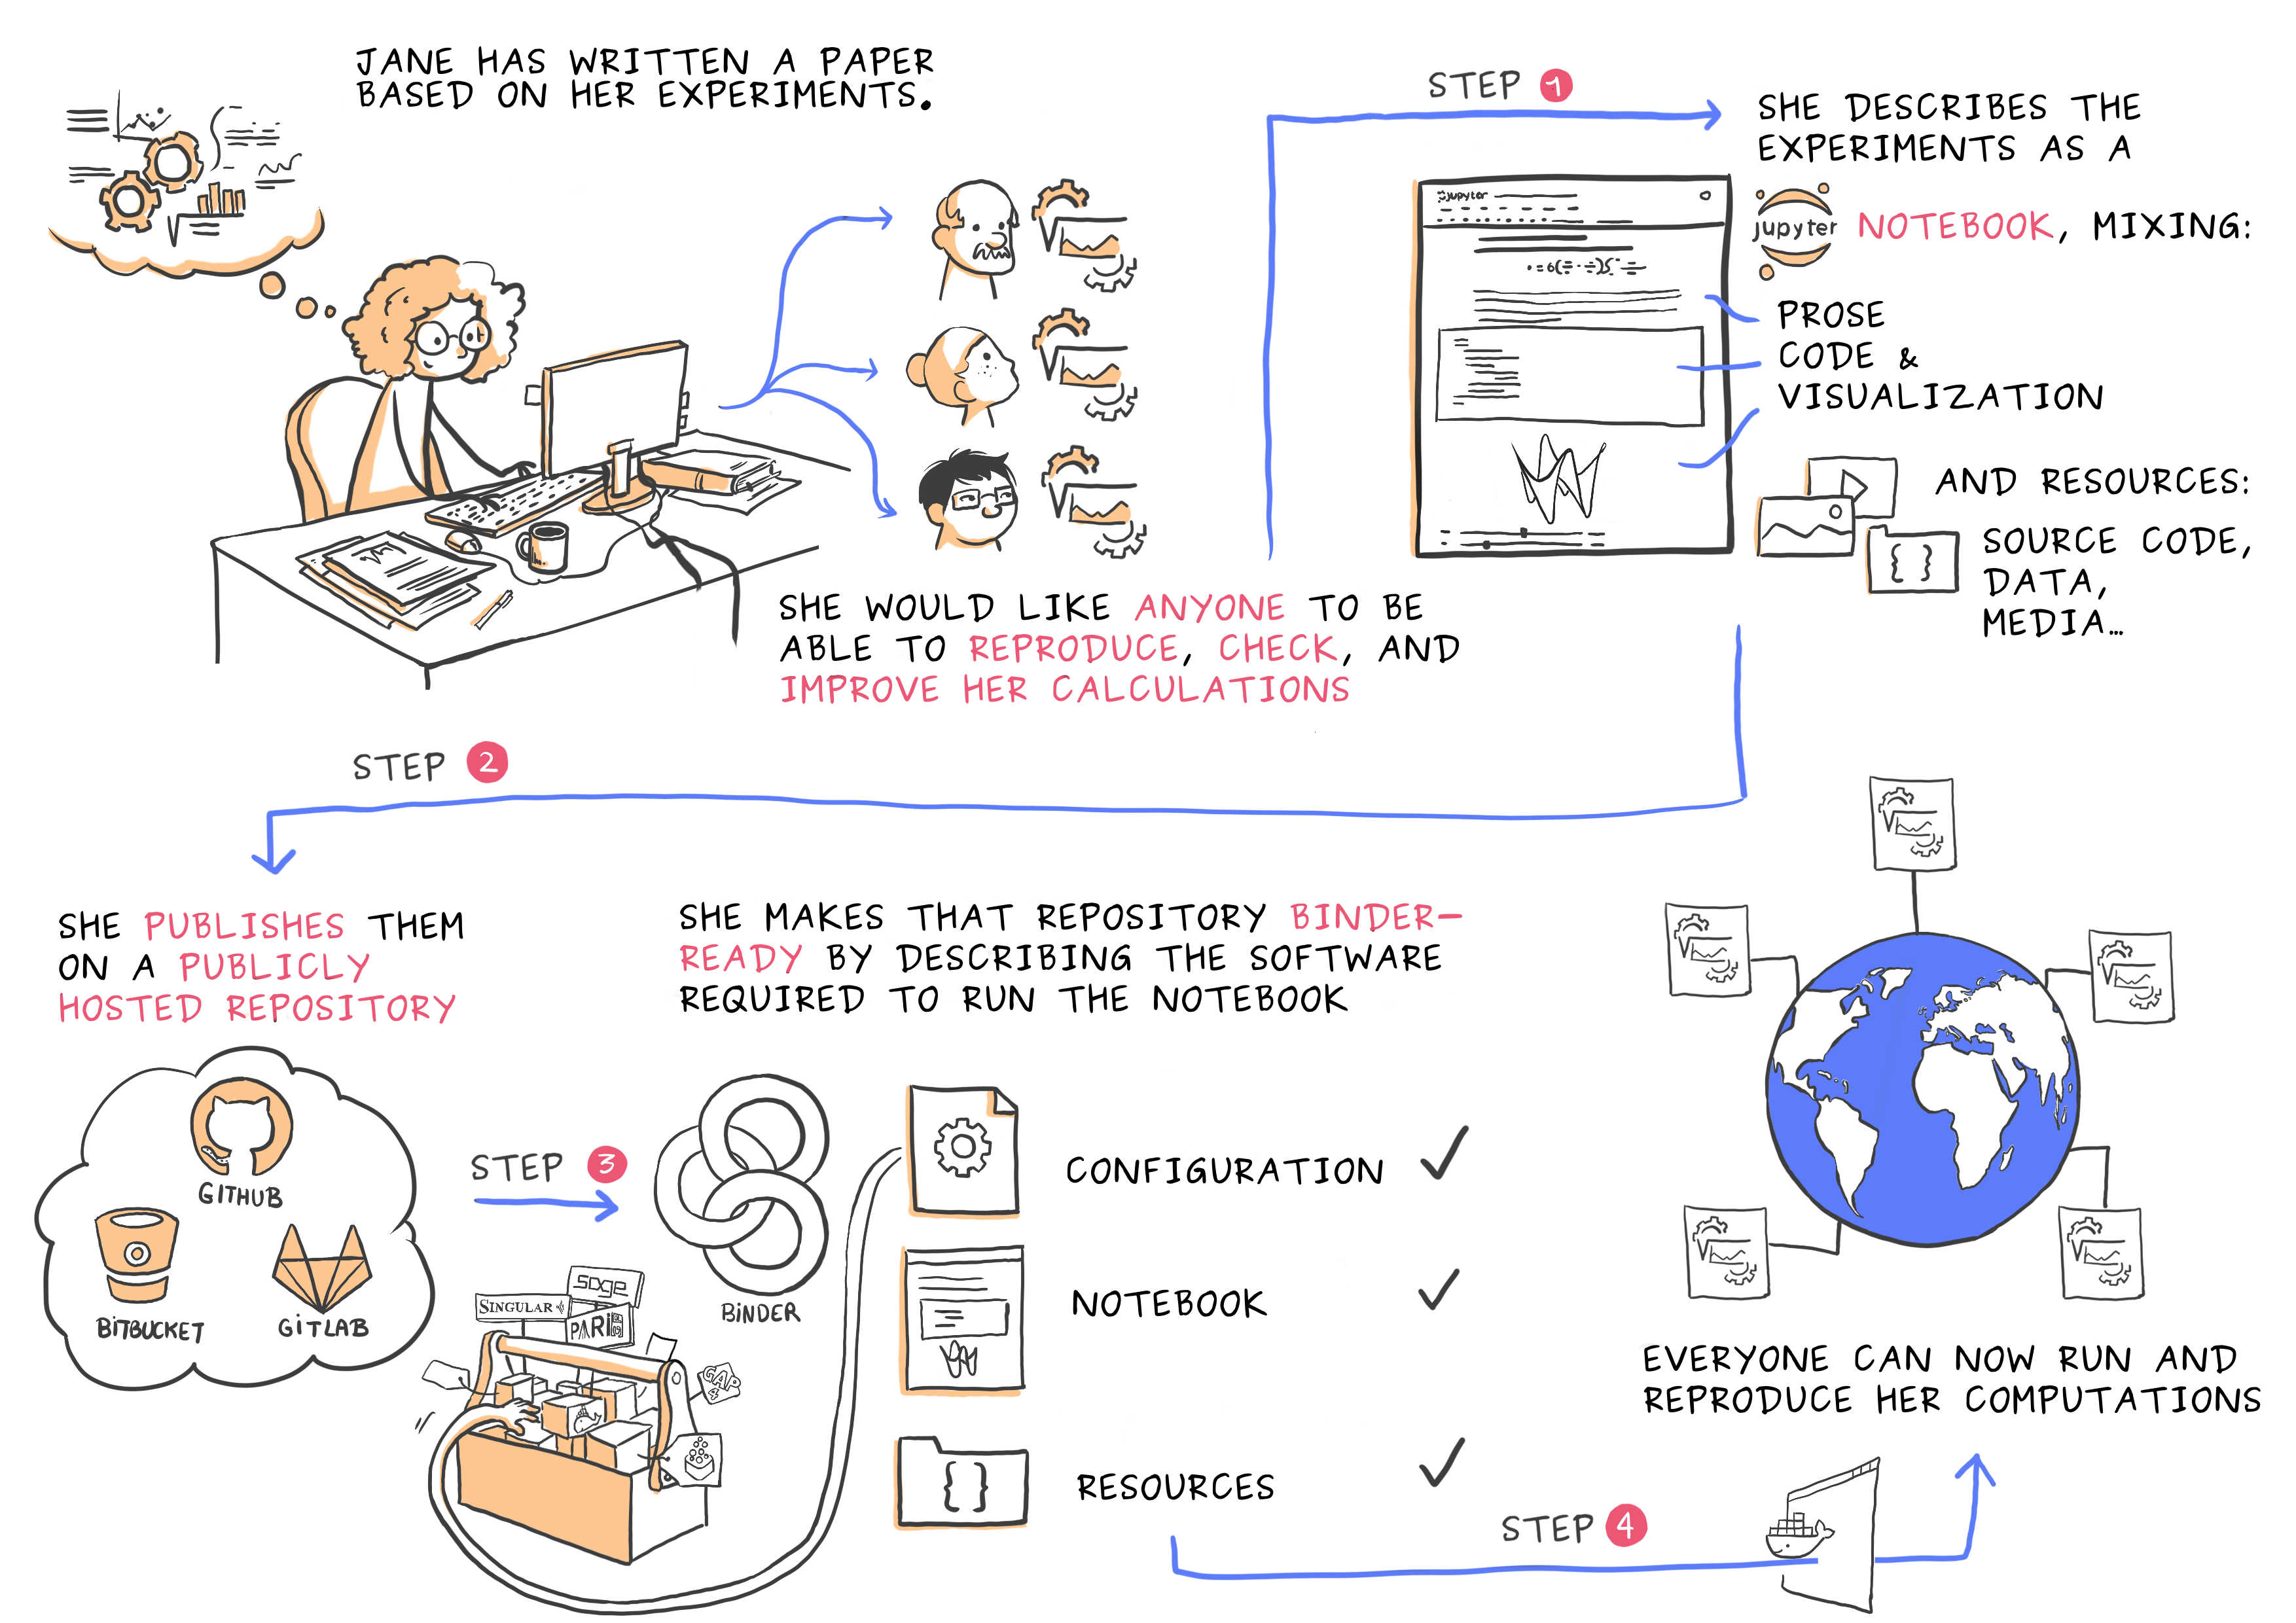
\includegraphics[width=0.9\textwidth]{use-cases-binder-logbook-solution.png}
  \caption{A typical use case for Jupyter notebooks in research.
            Image by Juliette Belin for the OpenDreamKit project, used under
            CC-BY-SA.}\label{fig:use-cases-binder}
\end{figure}

\TODO{
Structure as "The state of the art"
and "Above the art" for what BOSSEE will make better
}

Open Science is the principle that science, in order to be most
impactful and socially responsible, should be done publicly, with as
much of the scientific process and products accessible, reviewable,
and reusable by as many members of the global community as possible.
In the modern age of computational science, almost all academic
fields, from humanities to social sciences to biology and astronomy
are faced with exciting opportunities for Open Science.  As more and
more research takes the form of code and/or data, the opportunity to
share, reproduce, and reuse scientific work is greater than ever, even
enabling new forms of interdisciplinary collaboration.

At the same time as we share in these exciting opportunities, there
are corresponding challenges, technical and social, to making Open
Science a practical reality.  We face big questions: If a researcher
has code and/or data to publicise, how is that best done?  How do
researchers learn best Open Science practices in their field?  How do
previously disconnected fields benefit from each other's work as the
same computational challenges are faced again and again by different
communities?

These are the questions that guide \TheProject.
With so much research being done that wants to be Open,
how can we make Open Science

\begin{enumerate}
    \item as easy as possible to share?
    \item as useful as possible to other researchers and the public?
\end{enumerate}

\noindent Our plan for improving access and effectiveness of Open Science can be summarised as:

\begin{enumerate}
\item improve and maintain common software infrastructure used for
  Open Science
\item develop the Jupyter ecosystem to improve capabilities better
  serve Open Science
\item guide, validate, and demonstrate our developments through
  collaboration with a wide variety of application domains
\item enable students and researchers to perform Open Science through
  training and education, and improving inclusiveness by focusing
  these on under-served and under-represented communities.
\item operate services to facilitate Open Science collaborations with
  Jupyter software
\end{enumerate}

\medskip
\textbf{Jupyter ecosystem as the root of \TheProject}

\TheProject has chosen to centre its efforts on the Jupyter software
ecosystem.  The Jupyter notebook and Jupyter ecosystem is of
increasing importance in computational science and data science, in
academia, industry and services. In addition to supporting high
productivity of researchers, they have great potential to push open
science forward: the notebook provides a complete description of a
computational and data science study, and the notebook can -- in
principle -- be turned into a publication, or can be used to provide
the required computation for a part of a publication, such as a
figure. In this way, the notebook enables reproducibility of complex
tasks with hardly any additional effort on the user side (if used
appropriately). The Binder project allows to execute such notebooks in
tailored computational environments; an aspect of reproducibility that
is not widely supported yet. Furthermore, for users wanting to connect
to a local Jupyter notebook server on their machine, or to connect to
a server somewhere else on the Internet, the users only need a
webbrowser to display the notebook locally. Because of these
characteristics, the Notebook is already planned to become an
important service on the European Open Science Cloud (EOSC), for
example through the EOSC-04 funded PaNOSC project.

\TOWRITE{}{short definition of Jupyter components, mixing code \& prose, etc. }

Because the Jupyter notebook is a web-based application, it can be
deployed at computational facilities or in the cloud, and can function
as the basis for services exposing computational resources of all
kinds to researchers and the public.  Because Jupyter is
\textit{interactive}, it enables making scientific results and
communications more interactive than static publications.  The
audience can follow their own initiative and ask their own questions
of published data without needing support from the publishing author,
greatly facilitating the \textit{practicality} of Open Science.

\textbf{Jupyter is generic} \TheProject chose Jupyter because it is
Generic.  Jupyter makes no domain-specific or even language-specific
assumptions.  Any application where mixing description, code, and
results is valuable can make use of Jupyter.  This broad applicability
makes investment in the Jupyter ecosystem extremely effective, because
improvements to Jupyter can serve many communities simultaneously.

Jupyter is built from a collection of standard protocols and file
formats.  Jupyter is not just a single, monolithic piece of
software, but a description of how such software can be built.  The
result is the ability for a variety of communities and applications to
use components of Jupyter for their purposes, and/or reimplement pieces to
meet their needs.

For example:

\begin{enumerate}
\item The notebook file format is a well-specified JSON document,
  which can be interpreted by many systems.  This has facilitated the
  development of different services rendering notebooks, e.g. the code
  hosting website GitHub, which renders notebooks for easy viewing by
  anyone, without Jupyter software.
\item the Jupyter protocol describes how execution is performed, which
  has enabled the development of over one hundred kernel
  implementations in dozens of languages.
\item output in the Jupyter protocol uses web-standard MIME types,
  enabling any possible format to be an output in a Jupyter notebook.
\item the JupyterLab extension system provides a system for building
  applications from Jupyter components and others
\item the Jupyter Widgets provide a system for customizing and
  extending interactivity in Jupyter-based environments
\end{enumerate}

The popularity of Jupyter, with millions of users and hundreds of open
source contributors, indicates the value and impact of this approach.

\medskip
\textbf{Improvement to the Jupyter ecosystem}

The benefits of focusing our work on a mature system like Jupyter are

\begin{itemize}
\item vibrant community ensures health and sustainability
\item large existing user base maximises impact of contributions
\item mature software ecosystem maintains quality software through
  industry standards such as version control, tests, continuous
  integration, stable release cycles, roadmaps, and user support
\end{itemize}

The Jupyter community aims to be inclusive, and \TheProject will
continue this effort.  Jupyter is inclusive across a number of axes.
By being applicable across numerous domains, Jupyter and \TheProject
encourage participation from individuals of various interests and
backgrounds, and has taken action to improve diversity in the project
by participating in "Outreachy," a program of paid internships for
individuals from groups that face under-representation, systemic bias,
or discrimination.  Jupyter has also operated workshops focused on
training contributors from under-represented groups.  In being free,
public, open source software, Jupyter and \TheProject are accessible
to as many individuals as possible, and invites users and contributors
beyond origin, nationality, beliefs, orientation.  One area where
Jupyter has lacked in this regard is in the User Interface
accessibility, and we will help improve this in
\taskref{jupyter-core}{accessibility}.  Additionally, the project will
focus some of its workshops in \taskref{education}{workshops} on
under-represented communities.


\begin{figure}[ht!]\centering
  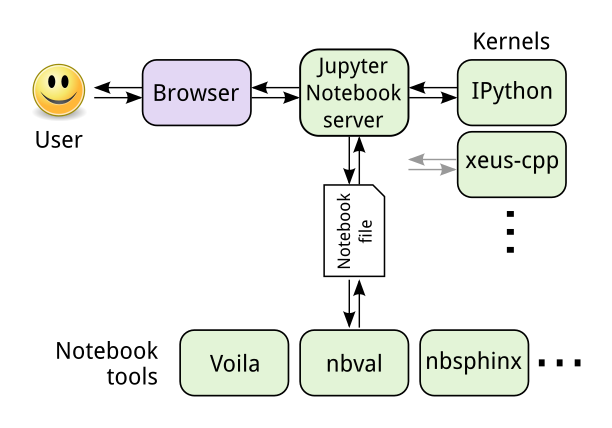
\includegraphics[width=0.6\textwidth]{images/notebook_components.png}
  \caption{The architecture of the Jupyter Notebook, kernels, and tools
        which operate on notebook files}
  \label{fig:notebook-architecture}
\end{figure}

\TODO{
  Architecture diagram of BOSSEE-related software
}

\medskip
\textbf{The science demonstrators}


\medskip

\emph{Demonstrator: Astronomy}

  The \href{http://cdsweb.u-strasbg.fr/}{Strasbourg Astronomical Data Center} (CDS) is scientific data
  center hosted by the Observatory of Strasbourg. The CDS plays a unique and
  essential role in astronomy by adding value to published and reference data.
  CDS runs astronomical services that
  provide data for the world-wide astronomy research community. Its three main
  services (SIMBAD, VizieR and Aladin) are heavily used with up to one million
  queries per day.  These services be accessed through web interfaces, mainly
  for human interaction, as well as through programmatic interfaces, including
  the standardized protocols defined by the International Virtual Observatory
  Alliance.

\begin{figure}[ht!]\centering
  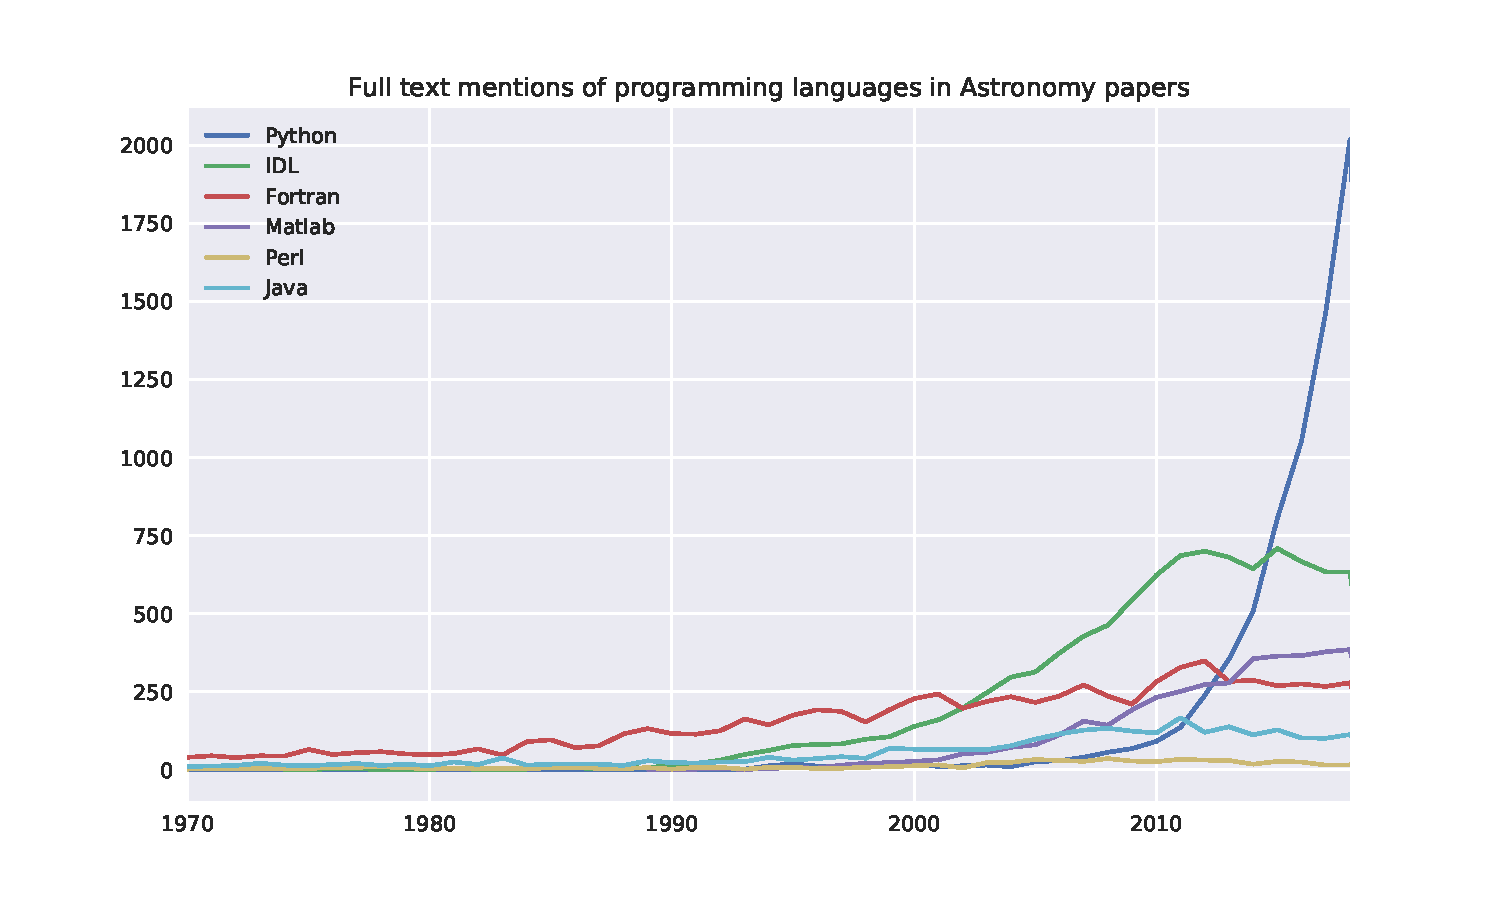
\includegraphics[width=0.6\textwidth]{python-astro-citations}
  \caption{Mentions of programming languages in refereed Astronomy papers, extracted from ADS. Python usage has increased dramatically in the recent years.}\label{fig:python-astro-citations}
\end{figure}

  Python and notebooks are rapidly increasing in importance for astronomy
  research. Indeed, Python for Astronomy software ecosystem has known a
  constant steady growth in the latest years, as shown in
  figure~\ref{fig:python-astro-citations}. As Python and notebooks integrate
  well together, the Jupyter notebook as an analysis tool is becoming a hot
  topic in the astronomical world: large surveys like the LSST (Large Synoptic
  Survey Telescope) have endorsed the usage of the Jupyter platform for their
    data access portal \cite{lsst2017scienceplatform}.\\


  We will develop a Jupyter-based framework to efficiently access, explore,
  visualize and analyze reference data that are available through CDS services
  as a real example of using open astronomy data.
  We will provide scientific users with a set of customizable Jupyter notebooks
  for visualization and analysis tasks, providing a new level of
  interoperability with python libraries and notebooks as is highly demanded
  by the astronomy research community.

  The focus is on the two following user stories:
    \begin{compactitem}
        \item analysis of catalogue data results, up to billions of rows.
              Tabular data is the typical output of SIMBAD and VizieR data.
        \item modular dashboard-like interface providing a top level
              interactive view of the available data for a given astronomical
              object and enabling loading and analysis of those data.
    \end{compactitem}


\begin{figure}[ht!]\centering
  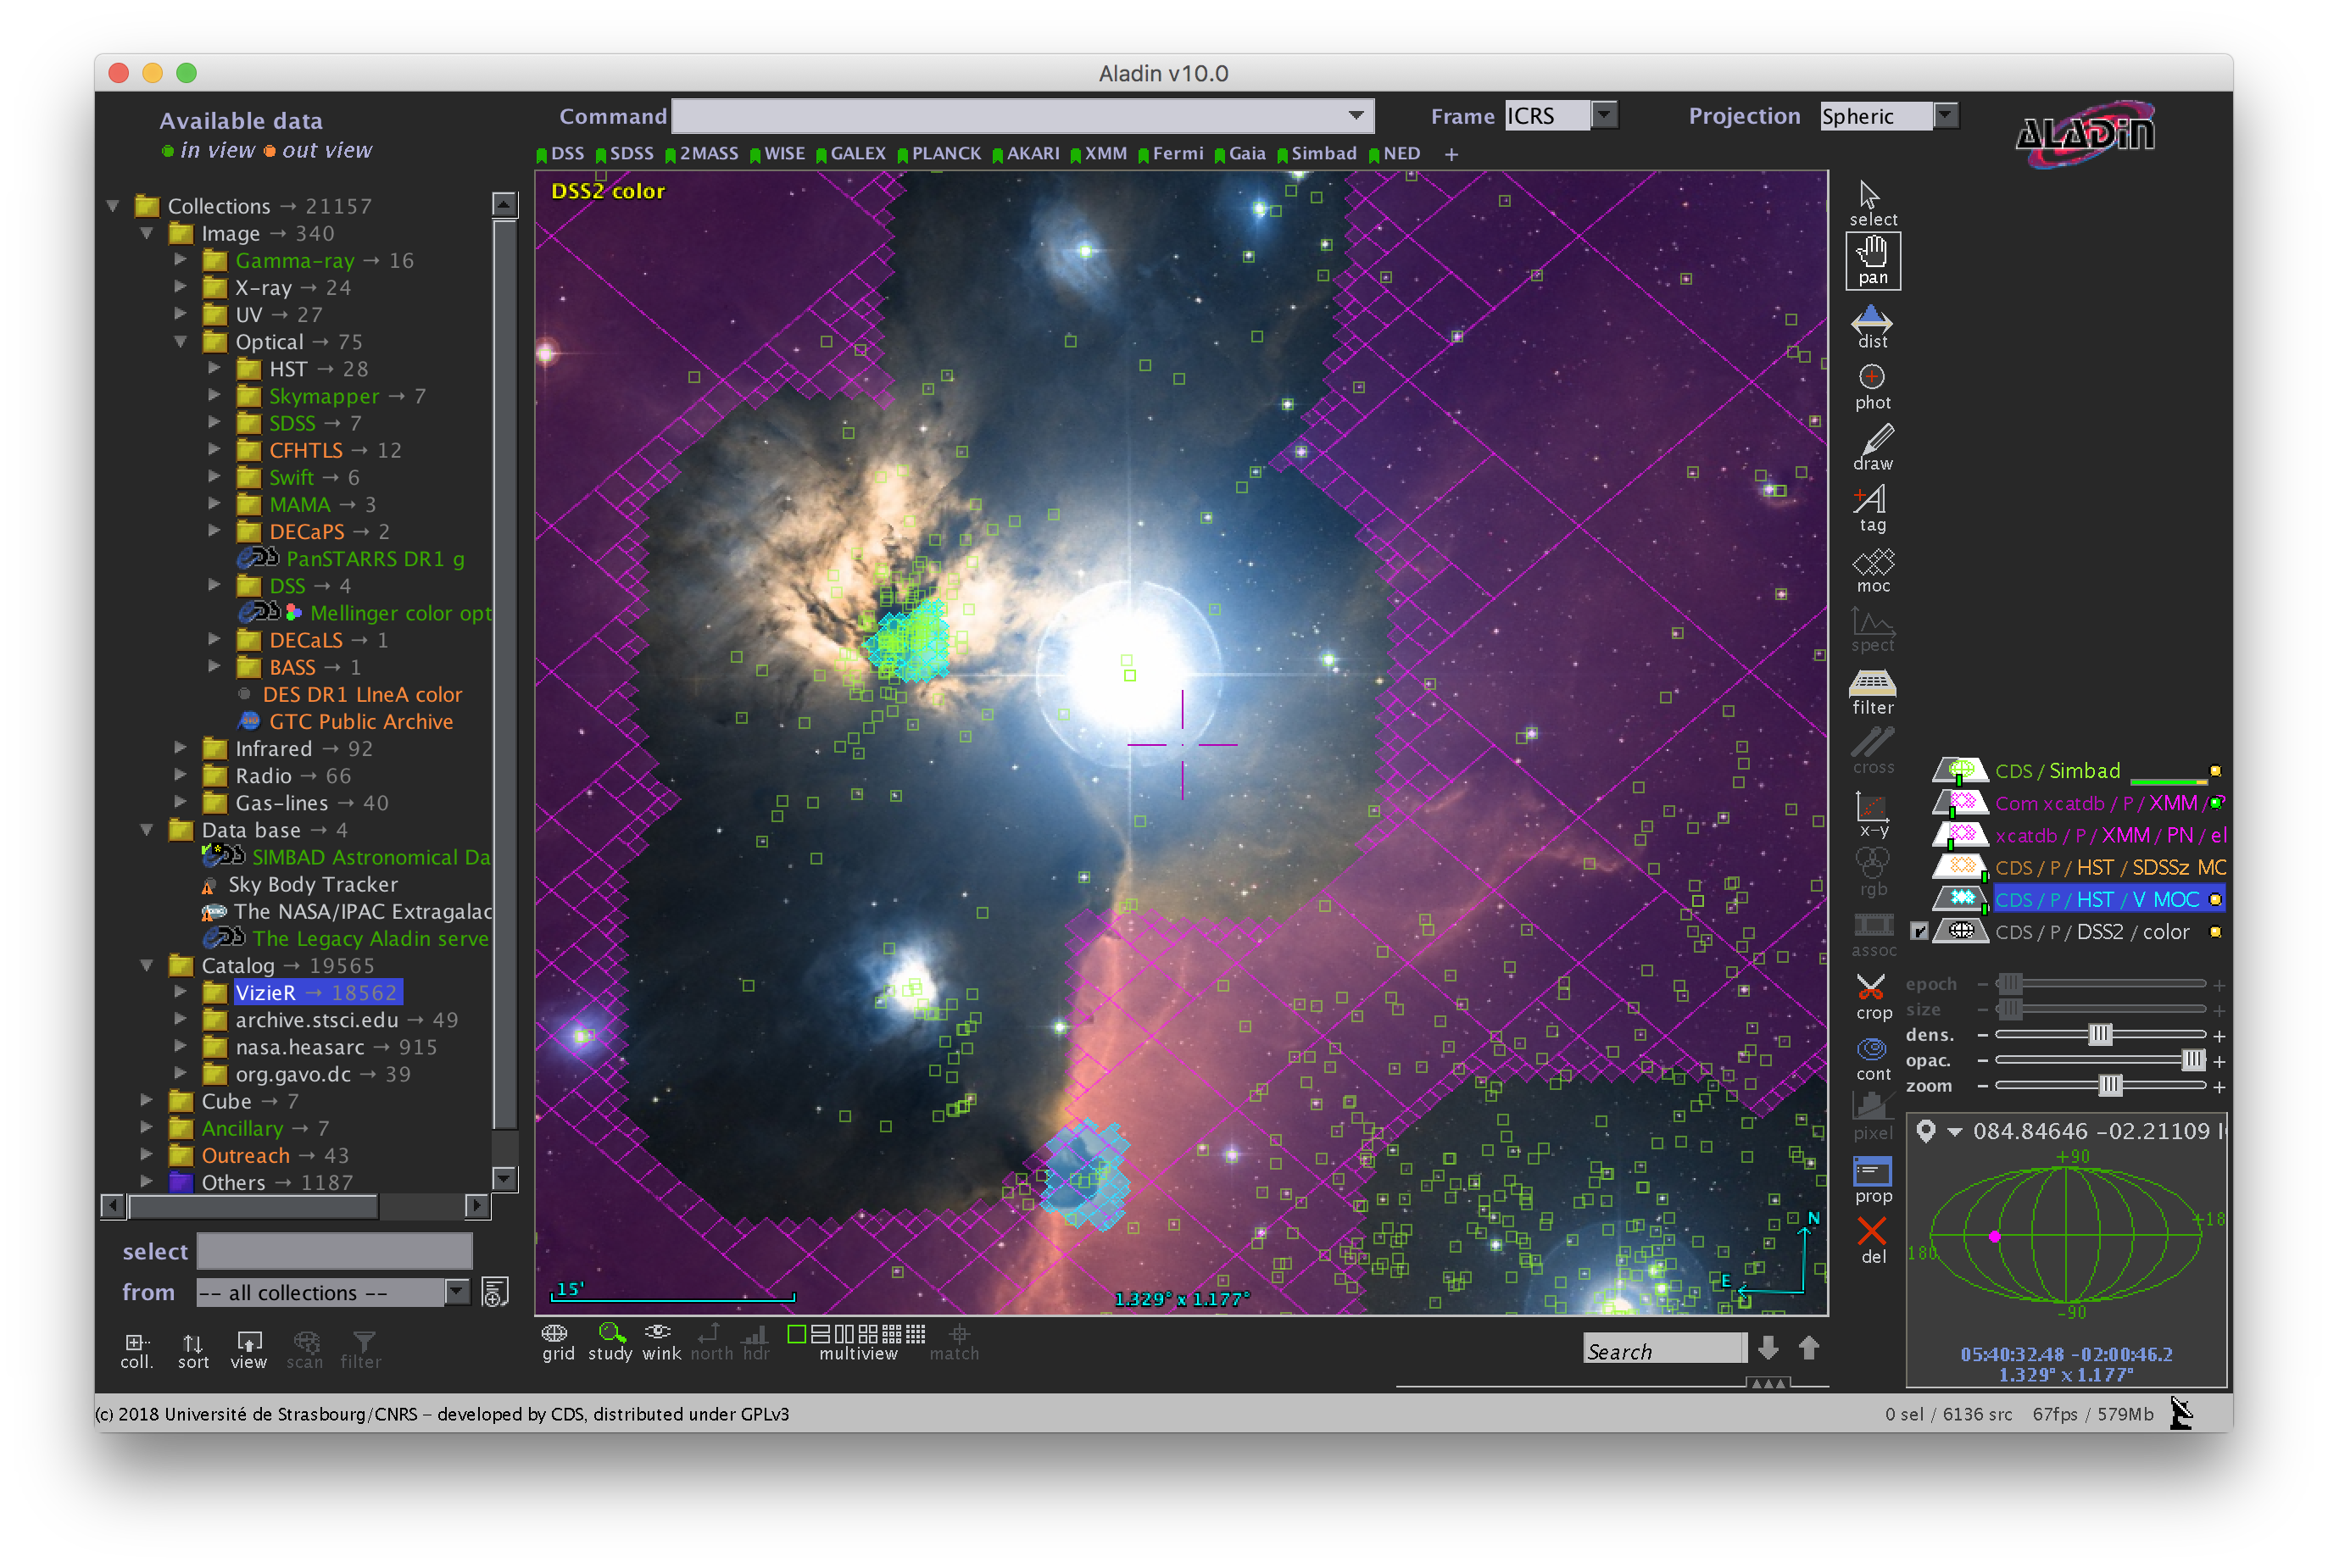
\includegraphics[width=1.0\textwidth]{astro-aladin-snapshot}
  \caption{Simbad objects, XMM and Hubble coverages overlaid on Digital Sky Survey imagery in the vicinity of the Horsehead nebula, and visualized in Aladin Desktop software.}\label{fig:astro-aladin-snapshot}
\end{figure}

  Access to the notebooks will be provided as a one-click action option from
  SIMBAD and VizieR results pages.
  Thus, providing with a one-click way of visualizing, filtering and analyzing
these potentially large tables will bridge the gap between access and analysis
of the data, with zero installation for the user.
  For specific science cases, we will explore rendering of notebooks with
  interactive widgets through "Voila", as to allow users not familiar with
  Python to benefit from the Jupyter notebook framework.
  Figure~\ref{fig:astro-aladin-snapshot} depicts typical data objects we want to analyse and interact with in the notebooks: images, catalogue data, datasets coverages.

  These new developments will be highly visible to the large number of astronomers who use the CDS services (50,000 unique visitors per month) and such tools are in high demand by these users.

  The CDS expertise in astronomy data and interfaces will be profitably combined with expertise of BOSSEE partners to ensure the deployment of high quality widgets (Simula, WildTree Tech, QuantStack).

\medskip
\textbf{Demonstrator: enriched teaching with Jupyter}

  As argued in Task~\taskref{ecosystem}{teaching-tools}, the Jupyter
  ecosystem offers a versatile environment which has been widely
  adopted in higher education in the recent years. École
  Polytechnique, Université Paris-Sud and other participants from this
  project have been early adopters (see the description of \site{EP}
  and \site{UPSUD}).

  \begin{figure}[ht!]\centering
  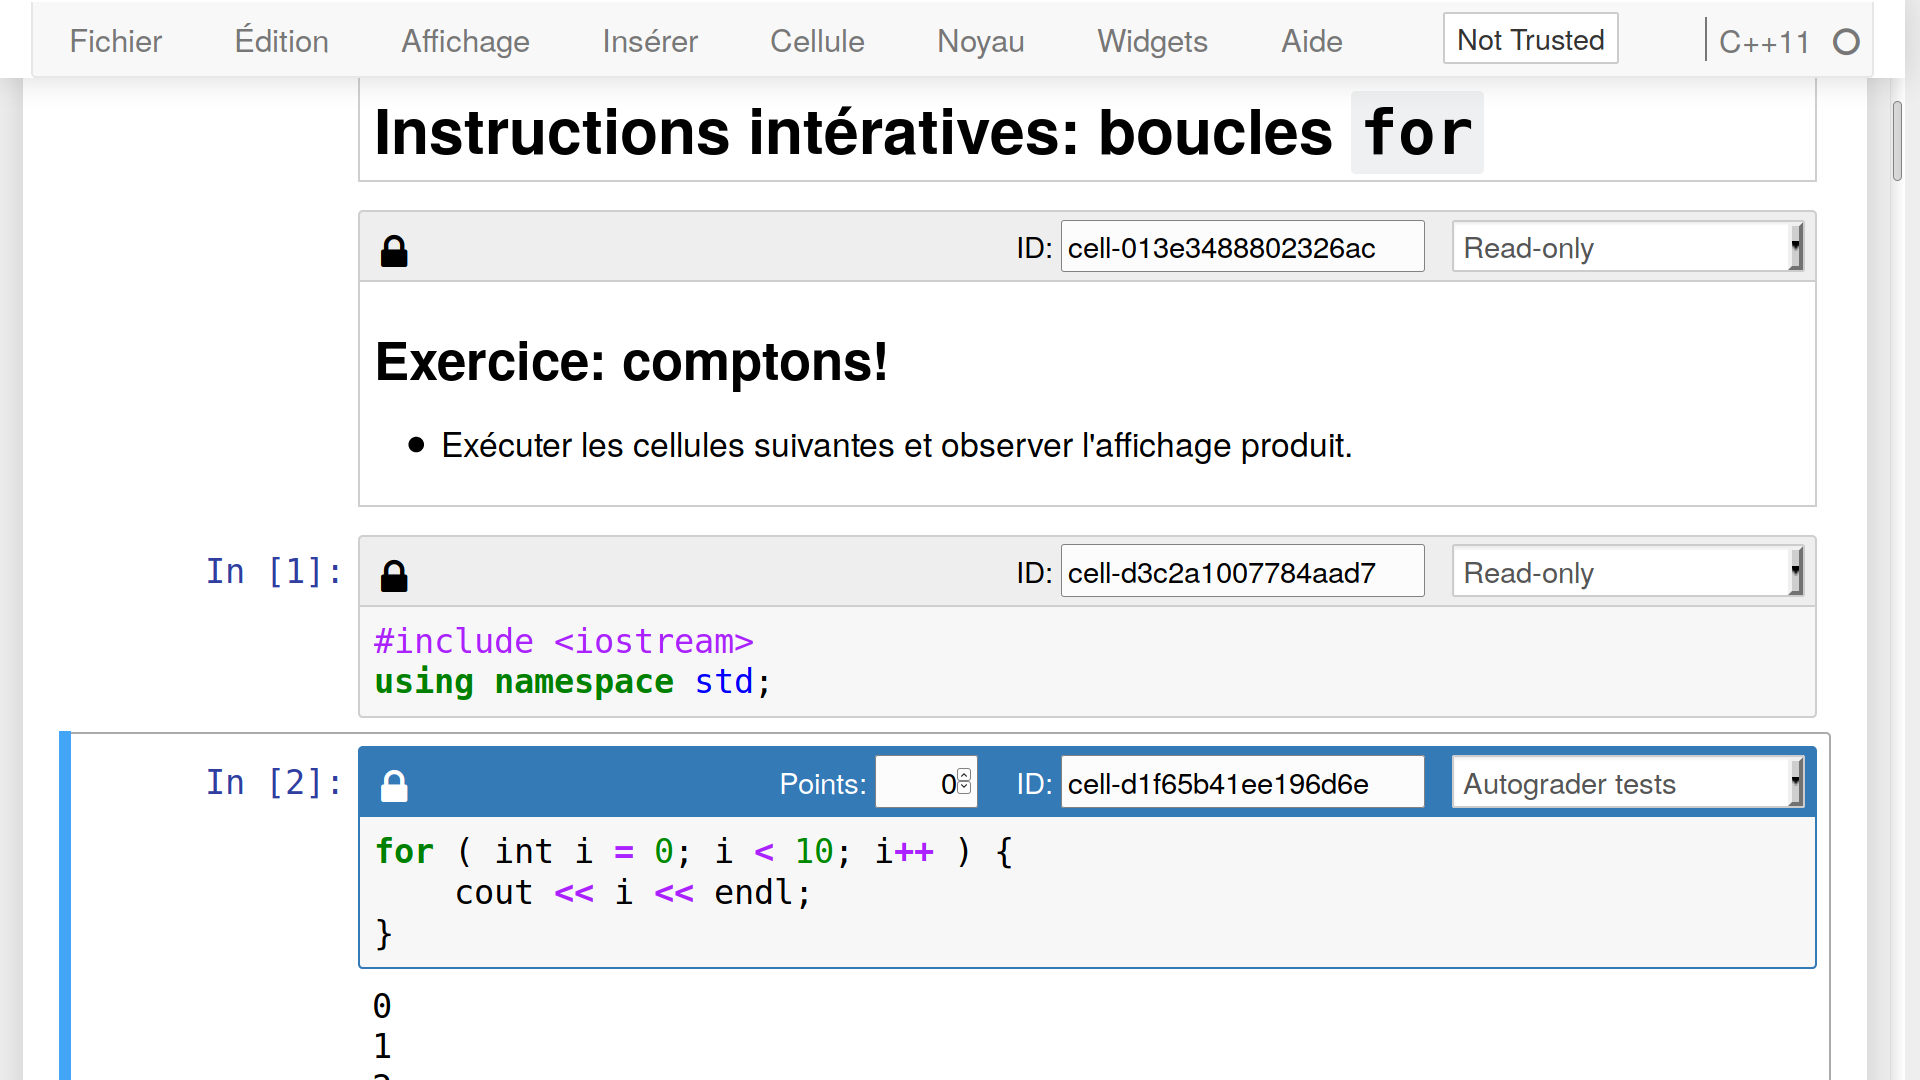
\includegraphics[width=.45\textwidth]{images/teaching-cling}\quad
  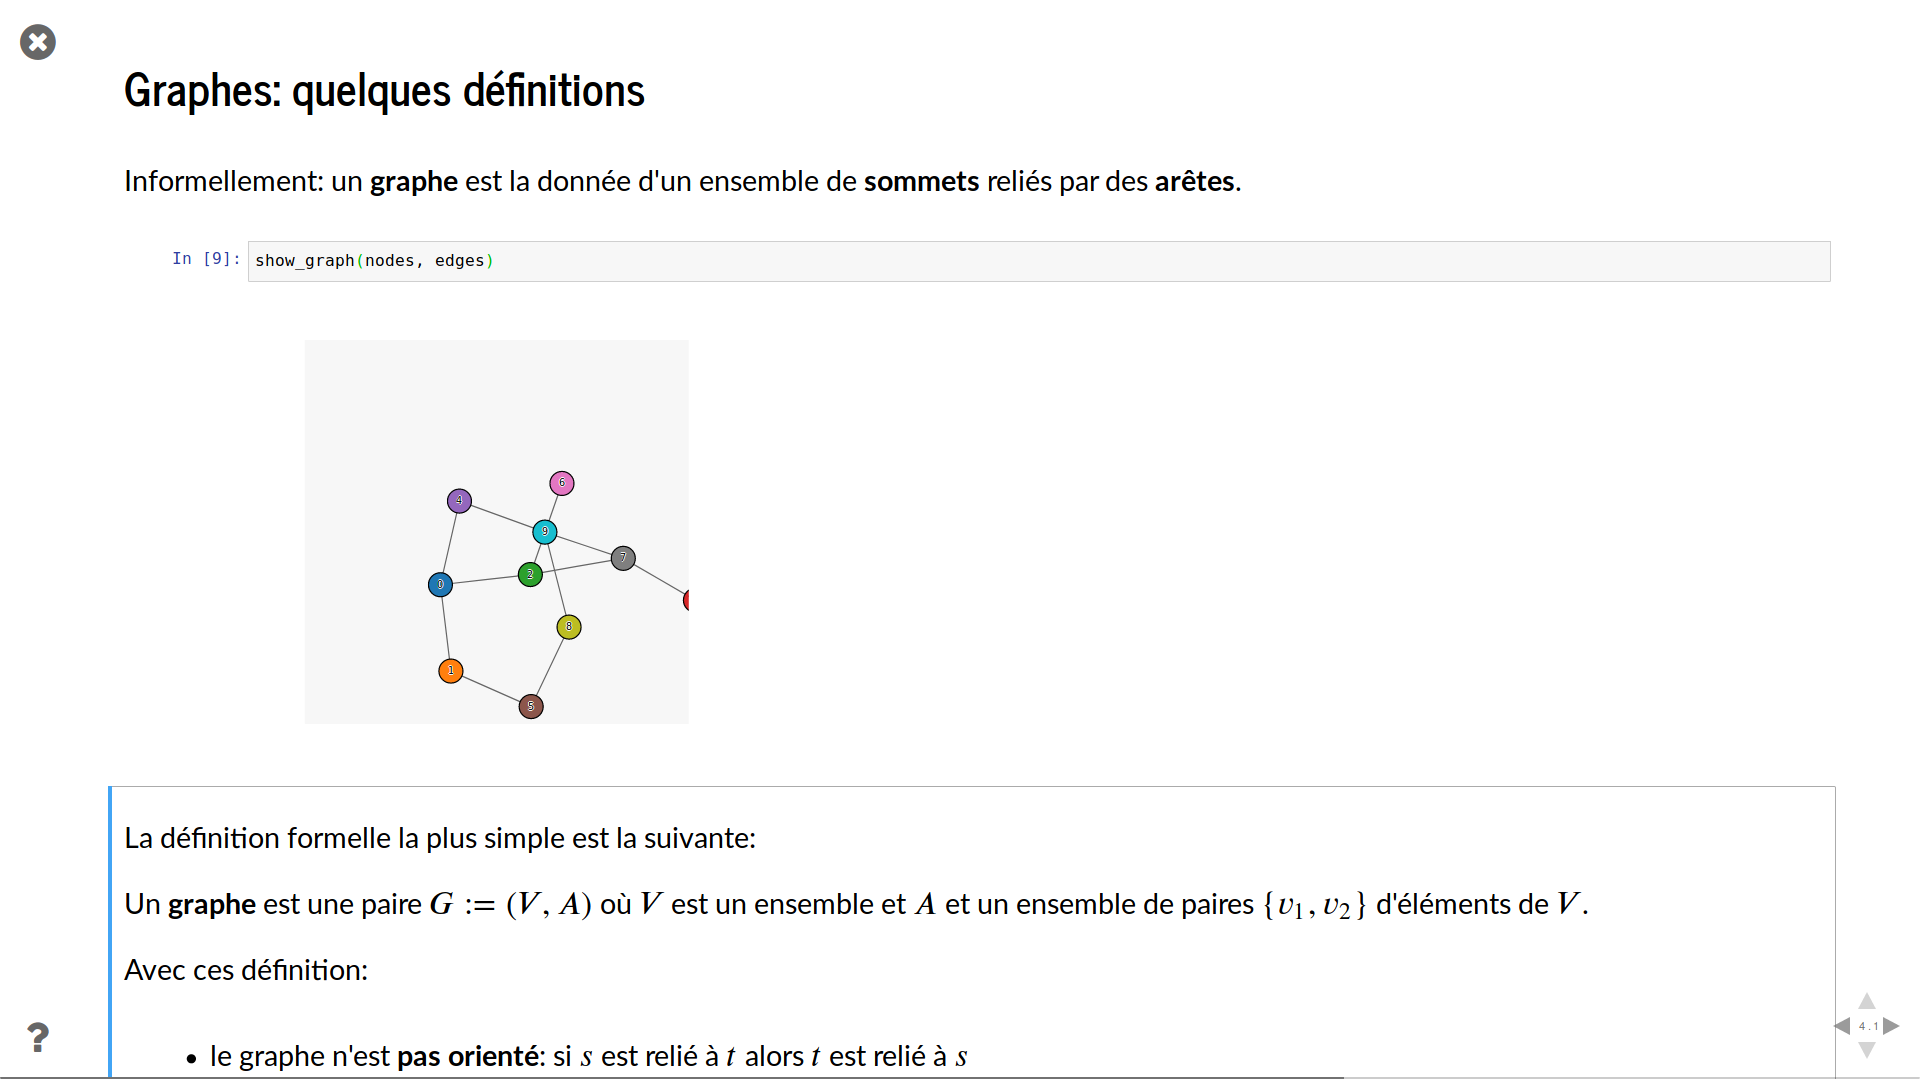
\includegraphics[width=.45\textwidth]{images/teaching-graphs}
  \caption{Jupyter based teaching material from Paris Sud. On the
    left: an exercise sheet for the course \emph{introduction to
      programming}; this instructor version showcases interactive C++
    execution and automatic grading configuration menus. On the right:
    interactive slides for a graph theory course.
    course.}\label{fig:teaching-cling}
  \end{figure}

  We learned the hard way that deploying the Jupyter environment at a
  large scale (e.g. for a university) requires specialized expertise
  (DevOps, software development, ...) which impediments its adoption
  by the greatest number of people. High quality hosted solutions
  (e.g. cocalc, gryd) do exist but are not the final solution when it
  is desired to get higher control on private data, integration with
  the local infrastructure (authentication, shared drive, e-learning
  environment, dedicated hardware, ...), or to use local computing
  resources rather than paid services.

  Further improving the Jupyter environment for education, while
  leveraging it to the greatest number, are therefore key motivations
  for the following tasks of this proposal:
  \begin{itemize}
  \item Tasks~\taskref{core}{jh-bh-conv}
    and~\taskref{eosc}{jh-bh-deployment} will greatly ease the
    deployment of Jupyter environments, with tight integration in the
    existing local infrastructure and full customizability by the
    teachers.
  \item Task~\taskref{ecosystem}{teaching-tools} will improve the
    interoperability with existing e-learning systems, and further
    develop teaching aids for, e.g., material sharing,
    (self)-evaluation, and grade management.
  \item Task~\taskref{applications}{math} will support teaching
    in mathematics through better support for real-time interactivity.
  \item Task~\taskref{ecosystem}{xeus-cpp} will support teaching
    in computer-science and scientific programming through
    better C++ integration in the notebook and will allow to first classe students to focus on the
    syntax of the language without distractions such as compiling and
    linking a program.
  \item Task~\taskref{eosc}{eosc} will ease publication and FAIR
    access to course material.
  \end{itemize}

\medskip
\textbf{Demonstrator: Visualisation and control of fluid dynamics in Jupyter notebook}


In recent years, the lattice Boltzmann method (LBM) emerged as an
interesting alternative to more established methods for fluid flow
simulations. Sailfish-cfd \cite{januszewski2014sailfish} is an open
source implementation of the LBM on General Purpose Graphical Processing
Unit (GPGPU) devices. It is written in Python with real-time
generation of CUDA-C code.  In order to harvest capabilities of GPGPUs
one needs to access the specialized hardware, which usually is
available to researchers as remote HPC resources.  The typical fluid
dynamics research workflow consists of three stages: preparing
boundary conditions, running a simulation, and data analysis. The
first and last stage require capable and responsive user interface for
maniputation and inspection of 3d data.  The Jupyter 3d visualisation
widgets developed in \taskref{ecosystem}{jupyter-widgets} can fulfil
such needs.

Based on previous experience with K3D-jupyter\cite{K3D}
widgets we know that web browser based software can display moderate
dataset during the simulation. As the dataset is becoming larger the
visualisation in the browser turns out to be nontrivial due to
limitations of the browser itself and required large data transfers. It is
an open question how much of data processing should be performed on
server-side and what can be done on the client hardware (i.e. in the
widget in the browser side of the user). Our
experience suggests that there is no clear answer and it depends on
the size of the data and its nature. For example, volume rendering
technique can be very effective on the browser side but infers large data
transfers. One can perform it the server-side, in a distributed way if
the simulation uses many nodes, but the interactivity is limited by
network latency. We will attempt to provide practical
solutions to this issue.
%

\medskip
\textbf{Demonstrator: Geosciences}

The amount of geospatial data from a variety of sources, including satellite observations, 4D simulations and in-situ observations, contributed by volunteers
or state agencies keeps increasing. In many disciplines, managing this large volume
has become a challenge, and the old approach of downloading datasets for a local
analysis has become intractable.

The heterogeneity of the tools used in different institutions to deal with
large geographical datasets makes it difficult for researchers to share the outcome
of their work in a reproducible fashion.

In this context, Jupyter is now emerging as a standard exploration tool for
geospatial analysis, climate science, geology and by data providers in these areas.

To mention a few,

\begin{itemize}
\item
   the \emph{PanGeo} platform \cite{Pangeo2018} (Funded by the NSF, NASA, and the
   Alfred P. Sloan Foundation) is built upon Jupyter, JupyterHub, Binder, and Dask.
\item
   the \emph{Joint Research Centre Earth Observation Data and Processing Platform}
   (JEODPP) \cite{Soille2018} relies on Jupyter, JupyterHub and ipyleaflet as
   its main user interface.
\item
   the \emph{Google Earth Engine} platform also offers a jupyter-based user
   interface allowing the visual exploration of the data with ipyleaflet
   \cite{GEEJupyterLeaflet2017}.
\end{itemize}

In these three cases, deferred processing is used to restrict computation to
the extent of the area displayed in the map viewer, which allowed these
platforms to scale up to petabytes of data. In all examples, interactive
visualization is a key feature of the platform. Beyond tile-based
2-D visualization, the ability to efficiently process and visualize vector
or 3-D  data is also becoming critical.

The BOSSEE team, which comprises the main authors of the technologies upon
which these platforms are built (Jupyter, JupyterHub, Binder, ipyleaflet),
together with the Department of Geosciences of the University of Oslo, are
in a unique position to bring these technologies together in the context of
EOSC.

This demonstrator will focus on tools for two transversal research projects

\begin{itemize}
\item LATICE (Land-Atmosphere Interactions in Cold Environments)
\url{https://www.mn.uio.no/geo/english/research/groups/latice/}
\item EarthFlows (Interface Dynamics in Geophysical Flows)
\url{https://www.mn.uio.no/geo/english/research/groups/earthflows/}
\end{itemize}

The work items for this demonstrator fall in two main categories:
visualization and geographical data processing tools.

\textbf{Teaching geo-sciences with Jupyter}

Beyond their use in scientific research, these development will be used in
the class room for teaching master's students with best practices in open
science.

\TODO{The transversal research plays into the desired ``services that
  encourate collaborative interdisciplinary work'' that are desired
  by this call; this is good. Can you imagine that some of these
  facilities can be used via the EOSC? That would be a good
  addition. For example, one could use the BinderHub installation
  that we expect on the EOSC. }

\medskip
\textbf{Demonstrator: Nuclear Medicine application}

  % Scientific description
  Nuclear Medicine is a field of medicine where radioactive material
  (radiopharmaceutical) is used for diagnostic and therapy. Even though the
  majority of Nuclear Medicine procedures (90\% according to successive EANM
  surveys) are diagnostic examinations, therapeutic applications tend to
  develop and drag more and more attention, for example for the treatment of
  neuroendocrine tumours \cite{Bodei2009}.

  The formalism used to objectively characterise the irradiation process is
  similar for both application types: it was introduced in the late 60s by the
  MIRD (Medical Internal Radiation Dose) committee of the American Society of
  Nuclear Medicine (SNM). This formalism \cite{loevinger1991mird} requires two
  independent quantities; the radioisotope cumulated activity ($Bq.s$) in the
  source (tissue/organ) and the mean absorbed dose to a given target
  (tissue/organ) per radioisotope disintegration (S-value,
  $Gy.Bq^{-1}.s^{-1}$). The S-value calculation requires a clear definition of
  the geometry of the patient (or the model) and radioisotope decay
  characteristics, it can be expressed as a linear combination of
  yields/energies ($J$) and Specific Absorbed Fractions (SAF, $g^{-1}$).

  The calculation of SAFs involves radiation transport modelling and energy
  deposition scoring in anthropomorphic models, usually based on Monte Carlo
  simulation. Historically, SAFs were computed from mathematical models -
  simplistic approximations to human geometry. The advent of voxel-based
  computational models requires a new appraisal of dosimetric data. For
  example, the models recently proposed by the International Commission on
  Radiation Protection (ICRP) include 140 possible radiation sources, leading
  to around 20000 source/target combinations \cite{ICRP2009ICRPPhantoms}. The
  production of SAFs for these models for all possible source regions,
  radiation types and energiesimpul represent an important computation time
  (millions of CPU hours).

  The OpenDose project \cite{Chauvin2017} is a collaborative effort to generate
  reference dosimetric data using various Monte Carlo codes across different
  teams. The collaboration includes at the moment 14 research teams over 18
  institutes.  The idea is to trigger the collaborative development of a
  reference database, freely available, proposing dosimetric data applicable in
  a context of nuclear medicine dosimetry (for therapy and diagnostic
  applications). A major aspect of the project is the development of tools
  ensuring traceability and reproducibility of generated results.

  % Technical description
  OpenDose data is produced using the five most represented Monte Carlo
  simulation software in medical applications: Geant4/GATE, MCNP, EGS, PENELOPE
  and Fluka. Each simulation consists of calculating radiation transport in
  anthropomorphic models for specific parameters (source organ, particle type,
  energy, model and number of primaries to simulate). Every simulation produces
  binary (3D matrices) and ASCII files for a total of $\sim$150MB / simulation.
  The 3D matrices contain energy deposited per voxels, and ASCII files contain
  pre-processed data corresponding to energy deposited per regions such as
  organs and tissues. These raw outputs are later processed into dosimetric
  data such as Specific Absorbed Fractions (SAFs) and S-values.

  Producing data for one model (ex. adult female) requires $\sim$30,000
  simulations, with the workload shared between the different teams and
  software.

  The data produced by all the teams is currently centralised at the Cancer
  Research Center of Toulouse (CRCT), processed and fed into a local SQL
  database at CRCT.

  This collaborative effort raises some challenges:
  \begin{compactitem}
  \item Data production: a total of 750,000 hours of CPU time is needed per
    model.
  \item Volume of data: one model represents TB of raw data that can be
    heterogeneous from the different teams.
  \item Data analysis: raw data has to be processed into dosimetric data in a
    robust and reproducible way.
  \item Database: has to be efficient and handle all the data (raw and
    processed).
  \item Visualization: display and compare results from all teams.
  \end{compactitem}

Figure
  \ref{fig:opendose_framework} shows the overall framework of the project and
  how data will be managed.

  \begin{figure}[t!]
    \centering
    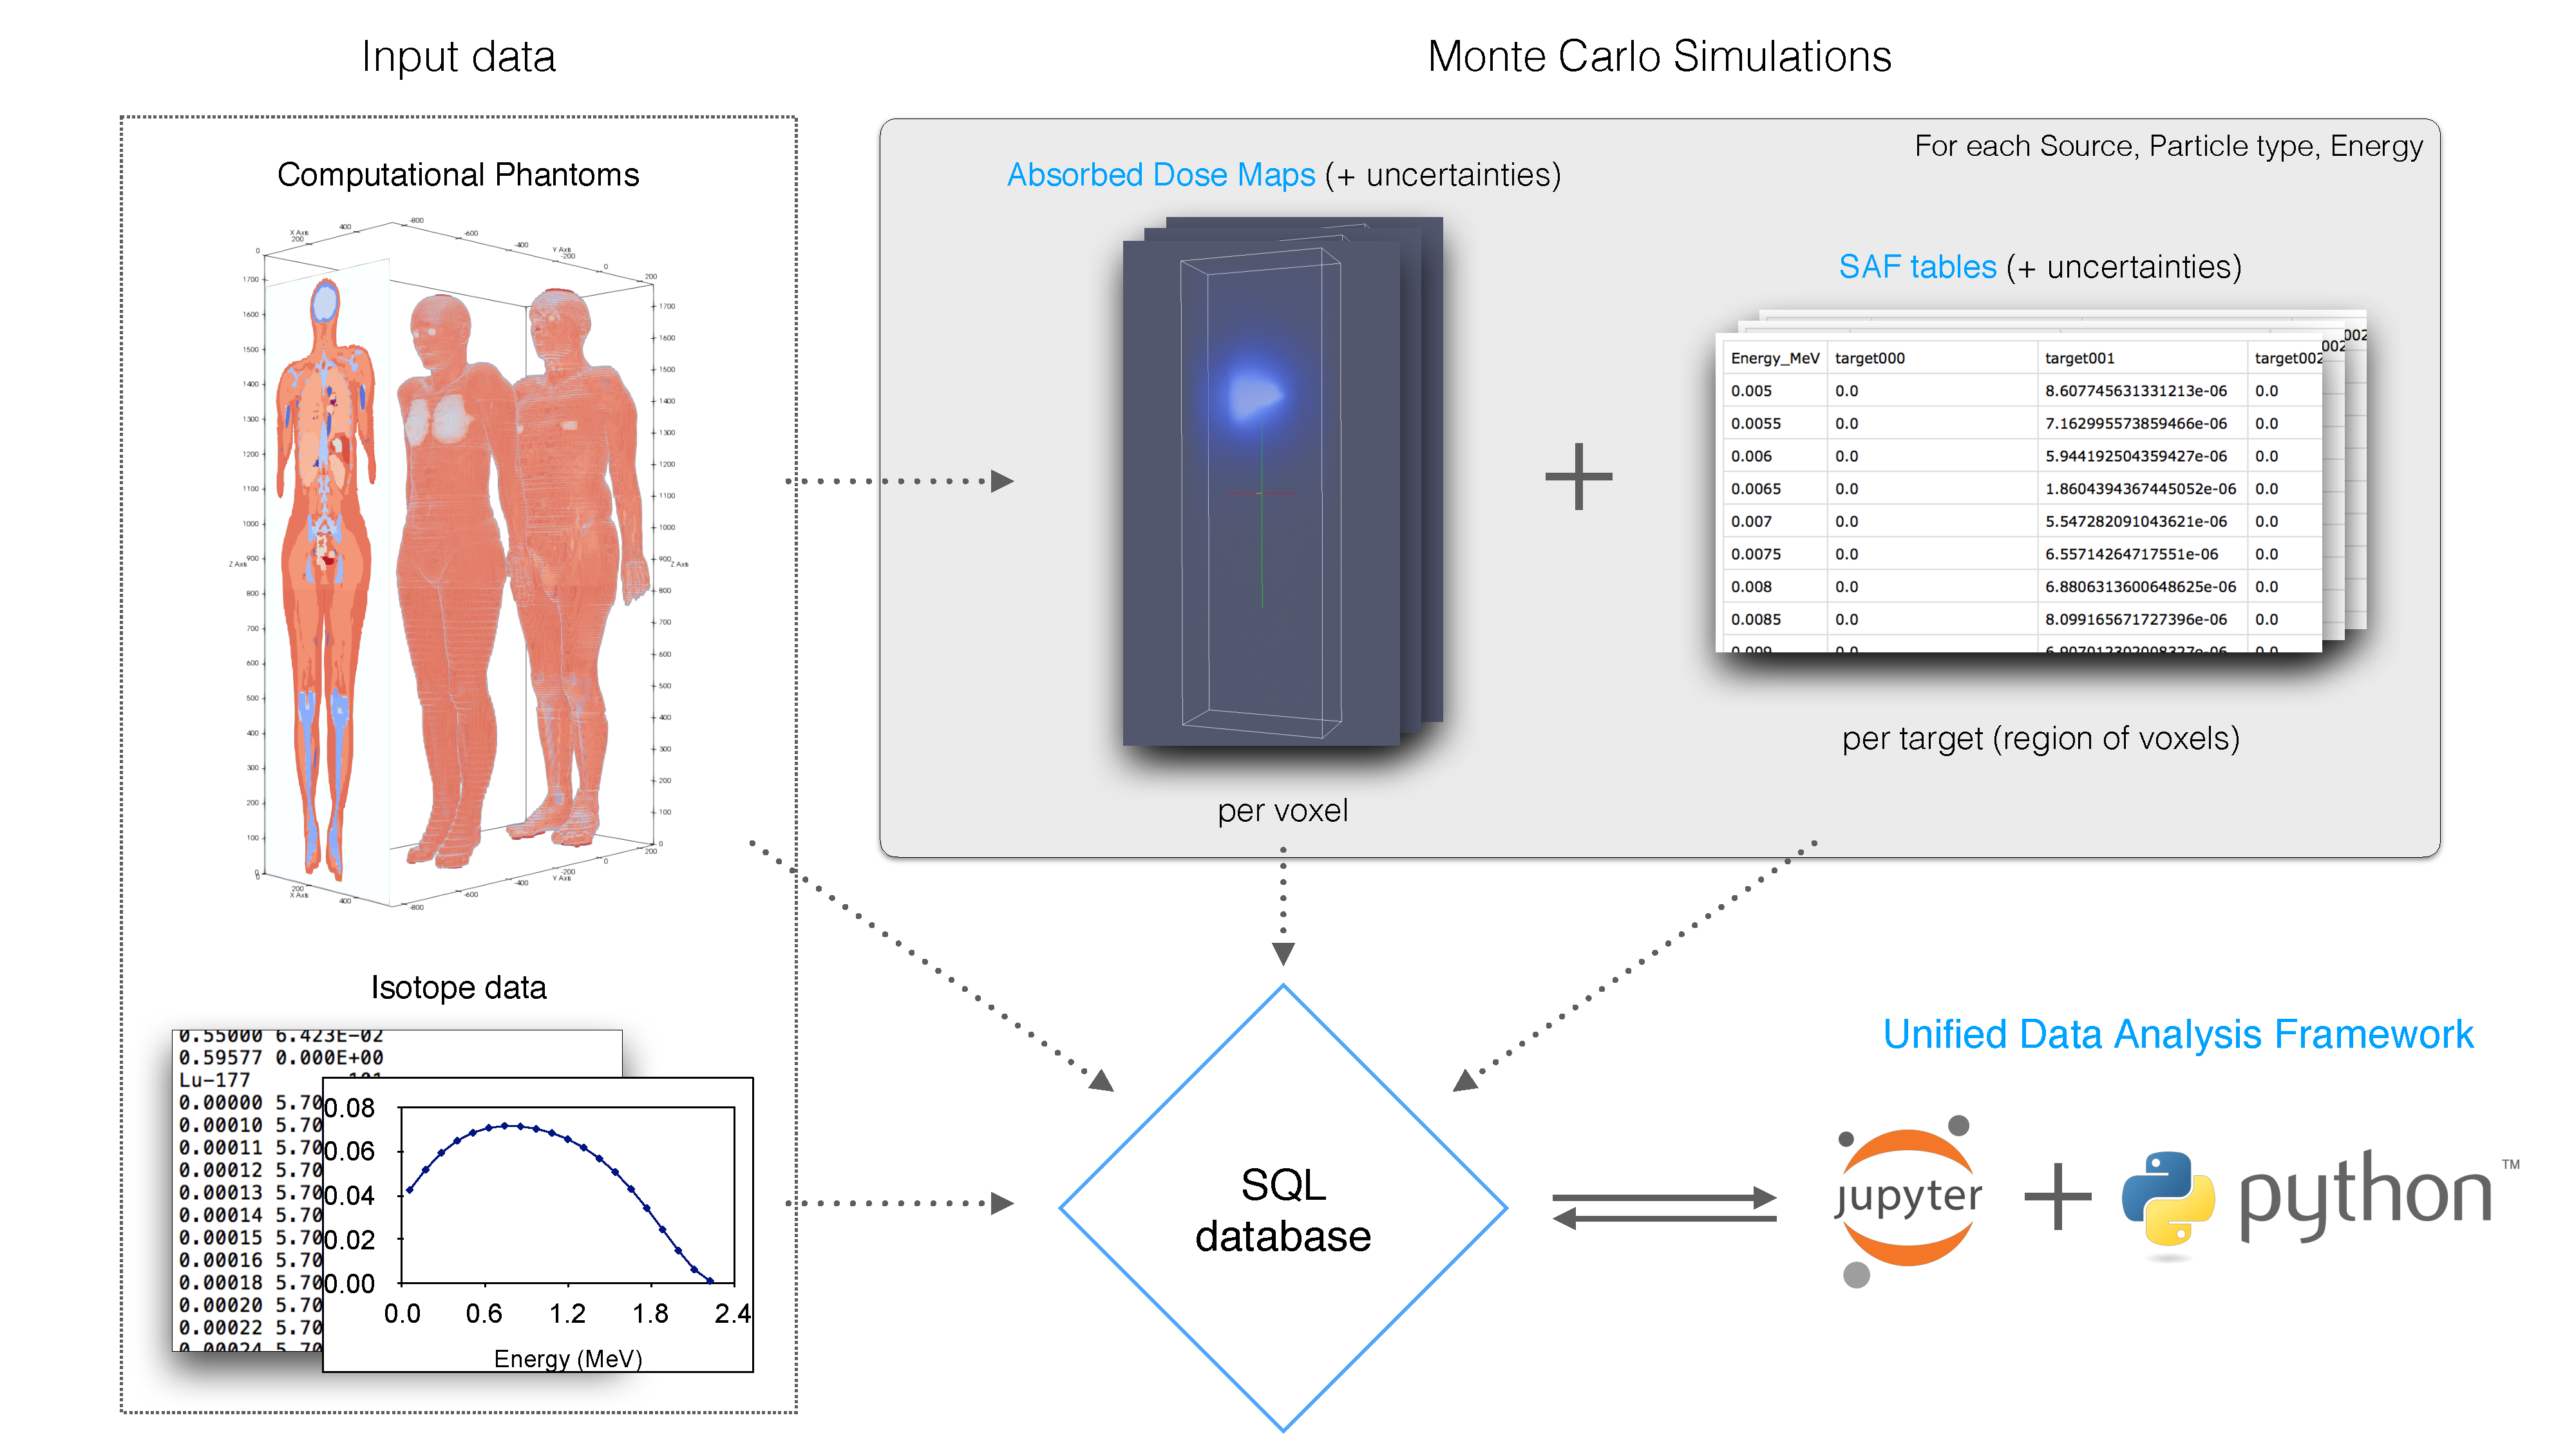
\includegraphics[width=1.0\textwidth]{images/opendose_framework.pdf}
    \caption{OpenDose project overall framework including the unified data
    analysis to be developed in this task.}
    \label{fig:opendose_framework}
  \end{figure}
  
  By building a set of tools to access and process data, this will ensure the
  production of traceable and reproducible dosimetric data for the OpenDose
  project members.

  Another major aspect of the OpenDose collaboration is to provide an open
  access to the generated dosimetric data. For that purpose a website is under
  development to allow data download and simple dosimetry calculations. For
  users who need more advanced calculations, a dedicated Jupyter workspace will
  provide a set of tools to easily access, process and display the OpenDose
  data.

\medskip
\textbf{Demonstrator: Interactive Mathematics with Jupyter Widgets}

  \TODO{Ideas to reinforce the ties with EOSC services welcome!}

  Computations have played a long time and ever increasing role for
  research and teaching in (pure) mathematics, to explore, search and
  check for conjectures, or better understand algorithmic ideas. This
  led to the development of a whole ecosystem of mathematical
  software, many of which are open source. Given the huge variety of
  mathematical objects and workflows, the Read-Eval-Print-Loop (REPL)
  paradigm -- on which Jupyter is based -- is particularly suitable:
  the user interacts with the system by typing commands that use its
  library of mathematical features, often combined with personal code.
  In fact, the REPL and notebook paradigms of Jupyter as well as some
  of its interactive features were largely inspired by that of
  computer algebra systems such as Maple, Mathematica, or SageMath.

  One major action of the OpenDreamKit project was to foster the
  convergence between the Jupyter and math software ecosystems:
  nowadays Jupyter can be used as a uniform user interface for most
  major systems: e.g. GAP, OSCAR, Pari/GP, SageMath, Singular, and
  even for C++ libraries. This interface is being widely adopted: for
  example, Jupyter has become the standard user interface for
  SageMath, enabling to phase out its former bespoke notebook; by now,
  thousands of jupyter notebooks for SageMath are publicly shared
  (6000+ on GitHub alone).

  Thanks to this prior art, the mathematical community will
  immediately enjoy all the benefits brought by EOSC-based generic
  Jupyter services, including eased collaboration, sharing, archival,
  and reproducibility.

  The next step to maximize attractivity and impact in the
  mathematical community, and this is the aim of this task, is to go
  beyond the REPL paradigm, and \textbf{leverage the real time
    interactivity and flexibility brought by Jupyter widgets for
    Mathematical purposes}. Think making it easy for a teacher or
  researcher to build and disseminate via the EOSC a mini applications
  or dashboard enabling the graphical exploration of a whole range of
  mathematical inputs, with real-time visualization of the associated
  outputs.

  The unique challenge comes from the huge variety of mathematical
  objects that the user may want to visualize and interact with, and
  the variety of graphical representations. Co-design is central here,
  as building a bespoke interactive visualization entails a
  combination of technology skills (e.g. javascript development) and
  business knowledge (designing the interaction and visualization).
  The role of Research Software Engineers is to leverage the
  technology by encapsulating the technical difficulties into flexible
  and easy to use tool boxes from which mathematicians can build
  mini-applications tailored to their needs.

  Within OpenDreamKit, we conducted experiments to explore this
  venue~\cite{ODK_D4.16}. One specific focus was to enable not only
  \emph{interactive visualization}, but also \emph{interactive
    editing}: being able to graphically modify the mathematical object
  being visualized; this enable the interactive exploration of how the
  modifications affect its properties, or to use the editor as input
  widget for a larger applications or dashboards. The outcome of this
  task are the development of two prototypes in SageMath
  (\software{sage-combinat-widget}, a library of widgets for
  combinatorics, and \software{sage-explorer} a generic dashboard for
  interactive browsing and introspection of mathematical objects), and
  contributions to \software{Francy}, an Interactive Discrete Math
  Framework for \software{GAP} and \software{SageMath}.

\medskip
\textbf{Demonstrator: Reproducible photon science workflows at European XFEL}


  European XFEL is a research facility that provides X-ray Free
  Electron Laser (XFEL) light to image structures at the nanoscale. It
  is currently the world's most brilliant laser, created in a 3.4km
  long tunnel, and supporting user experiments since September
  2017. These imaging capabilities from European XFEL and similar
  services from synchrotron and neutron sources, underpin lots of
  fundamental and applied research, in domains ranging from fundamental
  physics and material science to biochemistry and drug design. Some
  example data is shown in figure \ref{fig:photon-science-example}.

  All of the data recorded at European XFEL will be made freely
  available after an embargo period of three years
  \cite{EuXFEL-datapolicy-2017}. This provides scientific transparency
  and is expected to enable better exploitation of the data, as more
  researchers than those conducting the experiments have access to the
  results. If the analysis steps are not carefully recorded, there is a risk
  that the necessary understanding of the data is lost by the time it
  is made public or subsequently, greatly reducing its scientific
  value.

  We are keen to complement this open data access to the actual data
  with open access to reproducible data analysis, to confirm
  conclusions drawn and to significantly lower the barriers for
  re-analysis with new tools or for new research purposes.

  A task in the EC funded project Photon and Neutron Open Science
  Cloud (PaNOSC) is using the Jupyter Ecosystem tools as they are in
  2019 to provide interactive data analysis services to complement the
  data: through use of Jupyter Notebook and exploitation of the
  mybinder.org service, this activity will reduce the barrier for
  interactively exploring the data, understanding and making use of
  the data, and to do this through a central portal such as EOSC.

  Here, we combine and use the new developments of this
  proposal to enable new qualities of open science services, and to
  demonstrate the potential impact of these improvements for a wide
  set of EOSC services through a demonstrator in Photon Science.

  \medskip

\begin{figure}[tb]
    \centering
    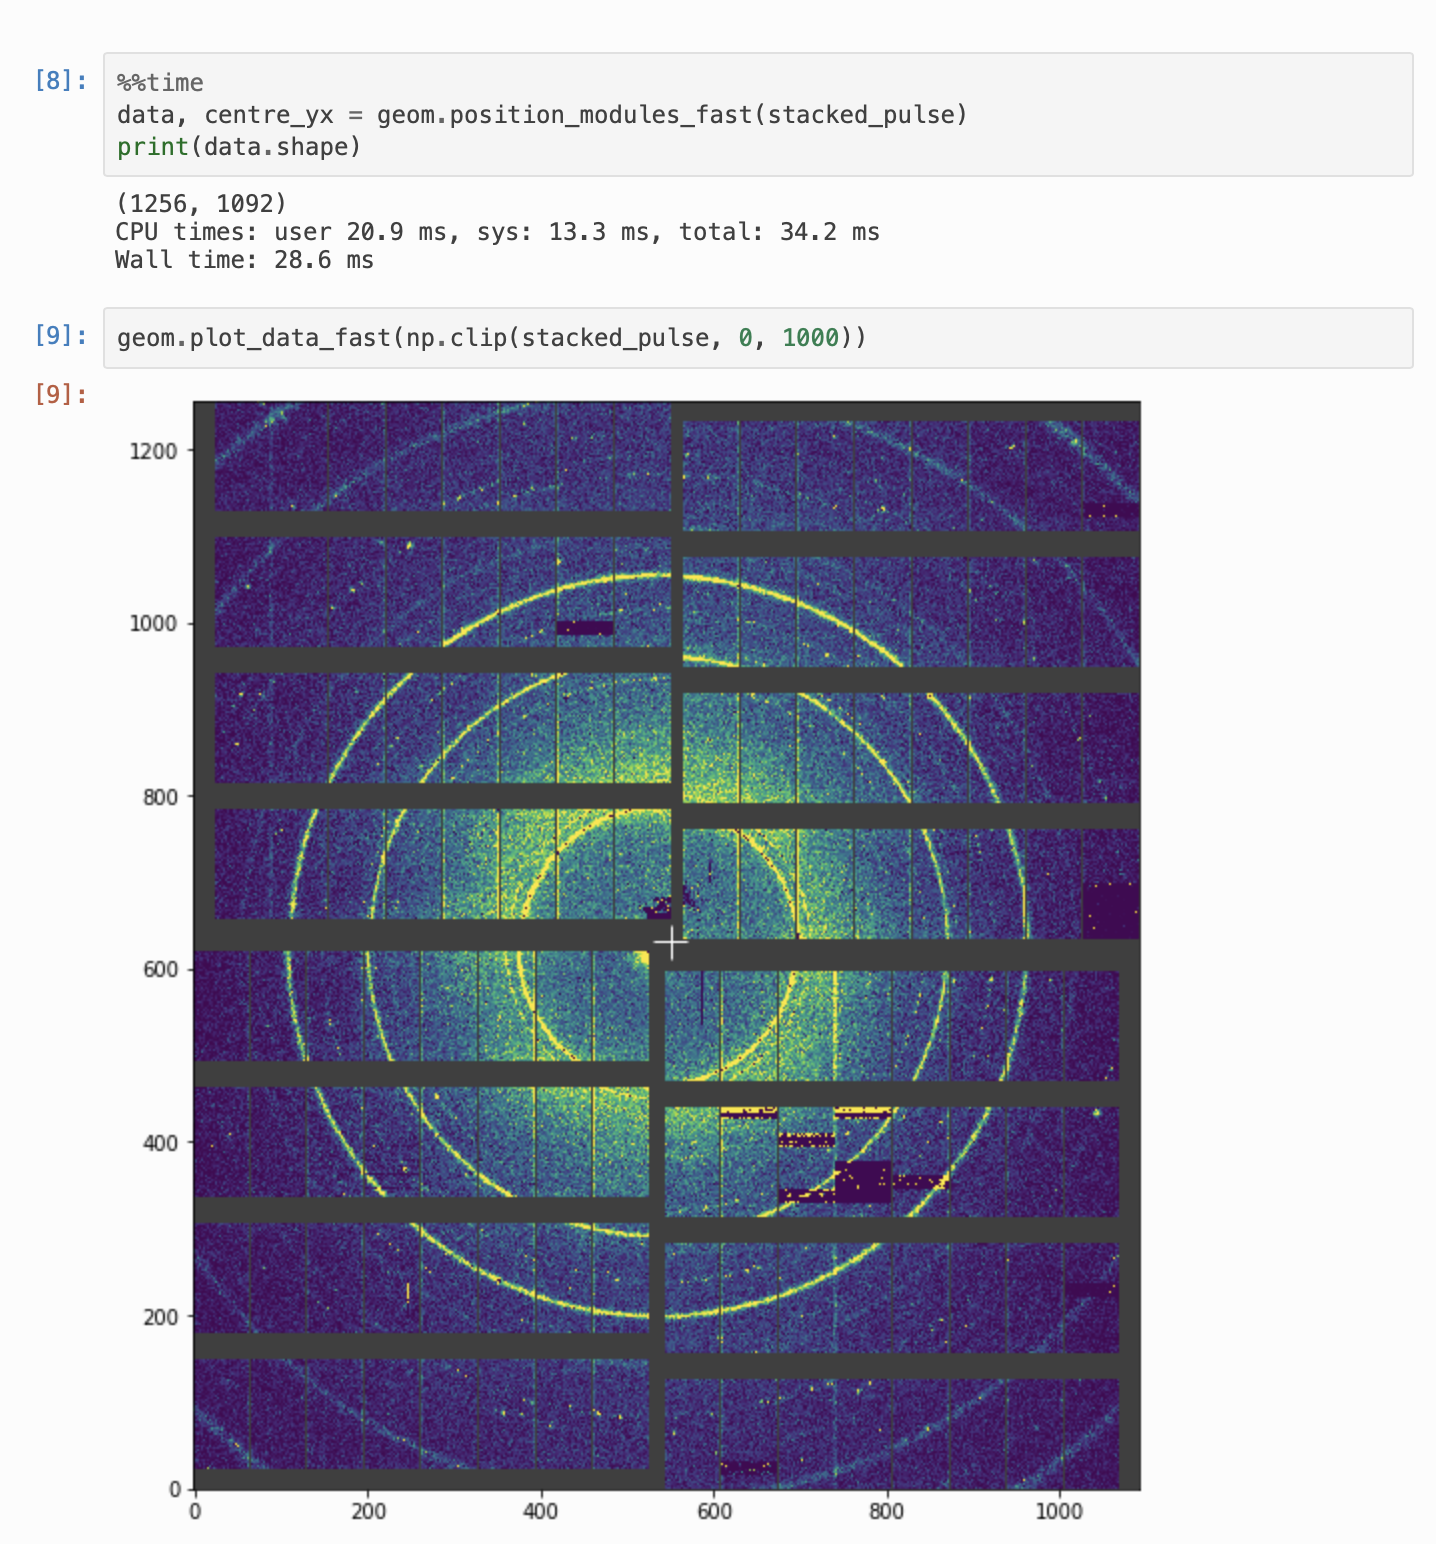
\includegraphics[height=0.27\textheight]{images/photon-science-prototype1.png}
    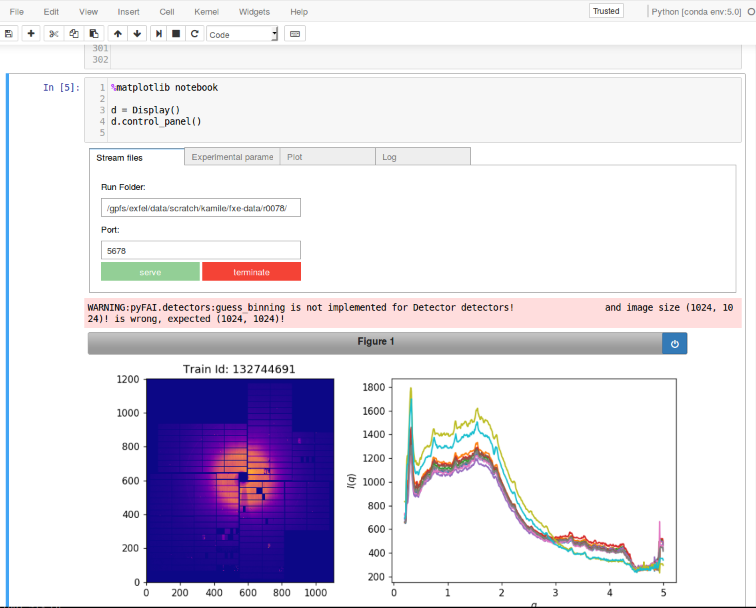
\includegraphics[height=0.27\textheight]{images/photon-science-prototype2.png}
    \caption{Prototypes for data analysis of 2d x-ray detector images
      in the Jupyter notebook, relating to the
      photon science use case.
      % task reference in caption doesn't work
      % \taskref{applications}{reproducibility-xfel}.
      \emph{(Left)} Data from crystallography
      scattering experiment. \emph{(Right)} Azimuthal integration of detector
      data as one step in the data analysis workflow.}
    \label{fig:photon-science-example}
  \end{figure}


  \textbf{Context}

  The very first experiments at European XFEL
  produced as little as 45 terabytes of data on average, but as the
  facility develops, the amount of data produced per time is expected
  to grow substantially: Given the rate of light pulses, there is the
  potential to produce up to a petabyte of data within the beam time
  of one experiment (typically one week). These significant amounts of
  data need to be complemented by complicated workflows to convert the
  data into insight through data analysis. Derived results of such
  data analysis are typically much smaller in size and useful to
  archive together with the raw data. To explain how they have been
  obtained, the particular workflow of data analysis also needs to be
  archived.

  \medskip
  \textbf{Vision}

  At European XFEL we will use Jupyter notebooks to facilitate
  this workflow: the simplest model would be to use one notebook per
  workflow. Once the data capture from the experiment is completed,
  this notebook can be executed (without being displayed in a web
  browser) to start processing the data. When the notebook has
  completed execution, it is saved, and contains the analysis results
  (it may of course also created files on disk as part of the
  process).

  A particularly useful aspect of the notebooks is that they mix data
  analysis commands with outputs, and that the notebook provides a
  complete (and thus reproducible) summary of the data analysis when
  it succeeds with the execution. Should the execution fail, for
  example half-way through the notebook, then derived results obtained
  prior to the error occurring are preserved and can be inspected. The
  error is embedded in the notebook and appears after the command that
  has triggered the error; which helps with debugging the process.

  This is of particular interest as the data analysis processes at
  European XFEL may fail not because of software errors but due to
  variation in the data that require (manual) expert adjustments of
  parameters. The ``failure'' of such an analysis workflow
  (represented through the Notebook) is thus not exceptional, but a
  common occurrence. The scientist conducting the experiment is
  sufficiently skilled to modify the parameters and wants to either
  re-execute the notebook from the beginning or to continue from the
  point of failure. The notebook caters for both use cases. The
  modified notebook would need to be preserved of course to provide
  reproducibility of the derived results that the notebook has
  computed.

  We are aiming for re-executability of the notebook for the lifetime
  of the data. The life time of the archived data at European XFEL is
  currently guaranteed for 5 years and aimed to be 10 years
  \cite{EuXFEL-datapolicy-2017}. It is possible though, that data used
  for publications will be preserved for longer, and it would be
  highly desirable to keep the data analysis re-executable for the
  same period of time, potentially well exceeding 10 years.

  \medskip \textbf{This task}

\subsubsection{Methodology}\label{sec:methodology}

\TODO{
 Explain the methodology in concrete terms. 
 For instance describe our roadmap for the service activities, networking activities and joint research activities.
 etc.
}

\begin{verbatim}
Outline notes:

* Carry on with specified protocols and formats so that components can be replaced, combined etc.
* Avoid lock-in to specific technologies (for example JupyterHub not limited to AWS but cloud-provide agnostic way) – thus independent from dominating commercial cloud services provider
* Integrating user input in multiple ways
   * User input at JupyterCon: beginners and experience users to try new version of UI; sessions where recorded and used to improve software (“usability testing”)
   * Co-design: developed by scientists for scientists, but professional software engineers and UX designers involved in the design of the software; [deliberate effort because Jupyter is a tool to teach beginners and specialists]
   * UI is at level of polish that is rarely met in non-commercial applications
\end{verbatim}
